\documentclass[tikz,border=4pt]{standalone}
\usepackage{amsmath,amssymb}
\usepackage{pgfplots}\pgfplotsset{compat=1.18}\usepgfplotslibrary{polar}
\usetikzlibrary{arrows.meta,positioning,automata,shapes,shapes.misc,calc,decorations.pathmorphing,decorations.markings,angles,quotes,patterns,mindmap,matrix,knots,hobby,trees}
\tikzset{->-/.style={decoration={markings, mark=at position 0.5 with {\arrow{Stealth}}}, postaction={decorate}}}
\begin{document}
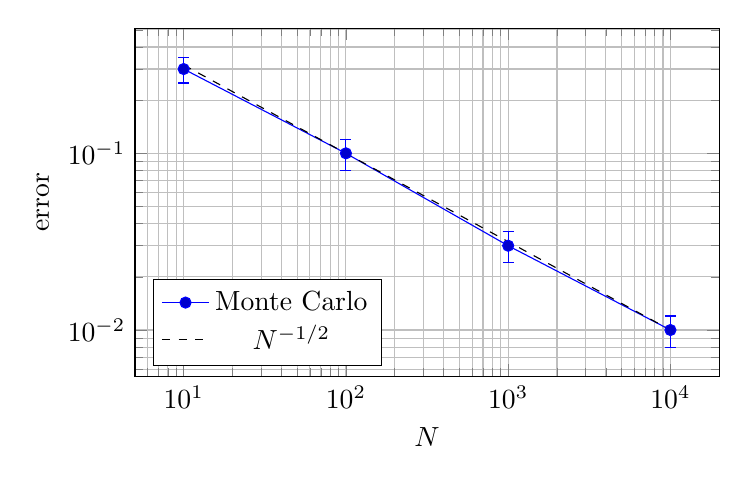
\begin{tikzpicture}
\begin{loglogaxis}[xlabel={$N$}, ylabel={error}, grid=both, width=9cm, height=6cm, legend pos=south west]
\addplot+[error bars/.cd, y dir=both, y explicit] coordinates {(10,0.3) +- (0,0.05) (100,0.1) +- (0,0.02) (1000,0.03) +- (0,0.006) (10000,0.01) +- (0,0.002)};
\addplot[dashed, domain=10:10000] {1/sqrt(x)};
\legend{Monte Carlo, $N^{-1/2}$}
\end{loglogaxis}
\end{tikzpicture}
\end{document}
